\subsection{Architekturdokumentation}
\label{architektur}

\subsubsection{Logische Architektur}
Wir teilen die Architektur des gesamten Systems in drei Schichten auf. In der Abbildung \ref{fig:architektur-methode635} sind diese als Presentation-, Businesslogic- und Persistence-Schicht zu erkennen.

\begin{figure}[h]
	\centering
	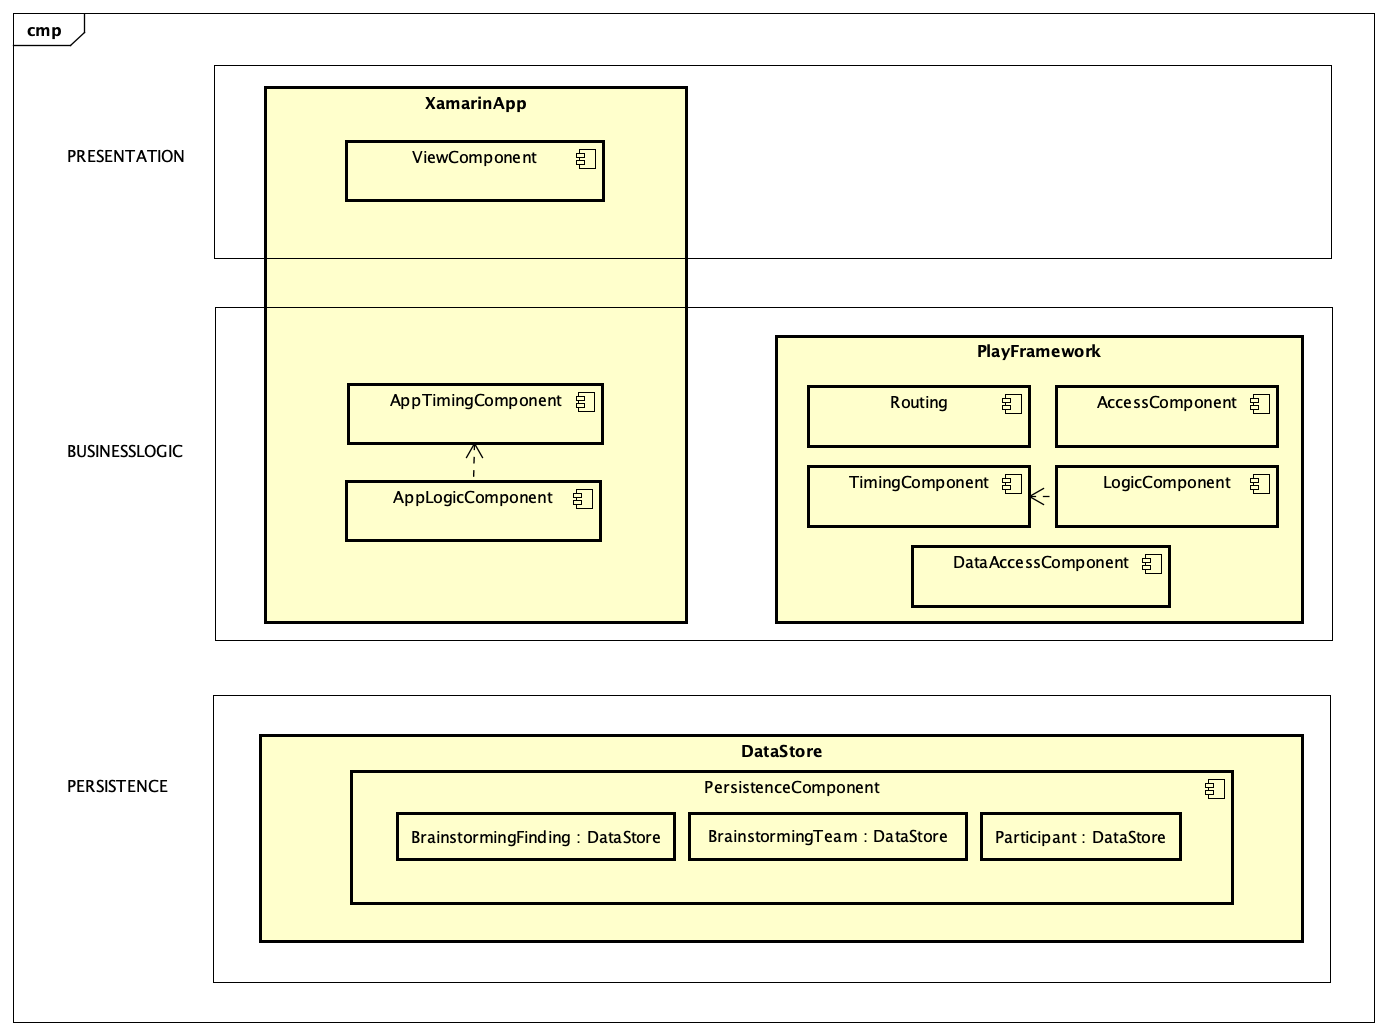
\includegraphics[width=1\linewidth]{img/architektur/CD_Methode635}
	\caption{Logische Architektur BrainingOutOfBox}
	\label{fig:architektur-methode635}
\end{figure}

Die Präsentationsschicht ist die Schicht über die der Benutzer mit der Xamarin App kommuniziert. Konkreter gesagt, umfasst diese die verschiedenen View-Komponenten, welche für das Aussehen der App verantwortlich sind. Jegliche Interaktionen über die Oberfläche werden anschliessend in der Schicht der Businesslogic weiter verarbeitet. In dieser Schicht haben wir zum einen wieder unsere Xamarin App, welche selbst Logik-Komponenten wie die Timing-Komponente oder weitere App spezifische Logik-Komponenten enthält.

Die AppLogic-Komponente ist für das korrekte Verarbeiten und Weiterleiten der Eingaben an das PlayFramework verantwortlich.

Die AppTiming-Komponente ist zuständig für das Zeitmanagement während den einzelnen Runden. Diese Komponente überwacht daher die noch verbleibende Zeit.

Auf der anderen Seite haben wir das PlayFramework, welches wiederum Access-Komponenten, Routing-Komponenten, eine Timing-Komponente, Logik-Komponenten und eine DataAccess-Komponente enthält.

Die Timing-Komponente und die Logic-Komponente haben die selben Aufgaben wie ihre Gegenstücke in der Xamarin App. Auch hier verwalten diese das Zeitmanagement während den einzelnen Runden und stellen sicher, dass nach Ablauf der Zeit oder sobald alle \textit{BrainSheets} abgegeben wurden, eine neue Runde beginnt. Des Weitern ist die Logic-Komponente zum Beispiel verantwortlich, dass ein \textit{Participant} einer Gruppe nicht zweimal beitreten kann oder diese verlassen kann, wenn er sie schon einmal verlassen hat. 

Die DataAccess-Komponente stellt sicher, dass jegliche Daten korrekt geladen oder gespeichert werden.

Mit der Schicht der Datenhaltung (Persistence) haben wir eine Schicht zur Verfügung, welche eine Persistence-Komponente hält. 

Konkret steht uns je ein DataStore für die \textit{BrainstormingFindings}, für die \textit{BrainstormingTeams} und für die \textit{Participants} zur Verfügung.


\paragraph*{Komponenten}
Nachfolgend sind nochmals alle Komponenten aufgelistet und kurz beschrieben. Für eine ausführlichere Beschreibung ist der Text oberhalb zu lesen.

\begin{description}[leftmargin=!,labelwidth=\widthof{\bfseries DataAccessComponent}]
	\item[ViewComponent] Die View-Komponenten der Xamarin App sind für das korrekte Anzeigen der Informationen verantwortlich. Sie definieren das Aussehen der Applikation.
	\item[AppTimingComponent] Die Xamarin App hält in der logischen Schicht eine Timing-Komponente, welche dafür sorgt, dass ein \textit{BrainstormingFinding} nach Ablauf der Zeit abgesendet wird.
	\item[AppLogicComponent] Die Logik-Komponente der Xamarin App regelt weitere Logik, wie z.B. den Zugriff auf das PlayFramework.
	\item[AccessComponent] Die Access-Komponente auf dem PlayFramework regelt den Zugriff mittels JWT-Token\cite{jwt}. JWT-Tokens werden bei erfolgreichem Login an den Benutzer der App gesendet. So kann sichergestellt werden, dass nur registrierte Benutzer mit dem PlayFramework interagieren können.
	\item[Routing] Die Routing-Komponente sorgt anhand der URL für das Aufrufen der korrekten Funktion.
	\item[TimingComponent] Wie die Xamarin App hält auch das PlayFramework eine Timing-Komponente, um den Zustand der Zeit verwalten zu können.
	\item[LogicComponent] In der Logik-Komponente werden die eigentlichen Funktionen geschrieben. Hier ist auch die Logik für den Austausch der Blätter untergebracht.
	\item[DataAccessComponent] Die DataAccess-Komponente stellt das Bindeglied zwischen dem PlayFramework und dem DataStore dar. Es ermöglicht erst den Zugriff auf die gespeicherten Daten.
	\item[PersistenceComponent] Die Persistence-Komponente regelt das korrekte und dauerhafte Speichern in die einzelnen DataStores.
\end{description}


\subsubsection{Deployment}
Wie in der Abbildung \ref{fig:deployment-methode635} zu sehen ist, besteht unser System aus zwei physikalischen Geräten. Das ist zum einen der Client und zum anderen der BackendNode. Diese beinhalten jeweils sogenannte \textit{DeploymentUnits} (DU). 

\begin{figure}[h]
	\centering
	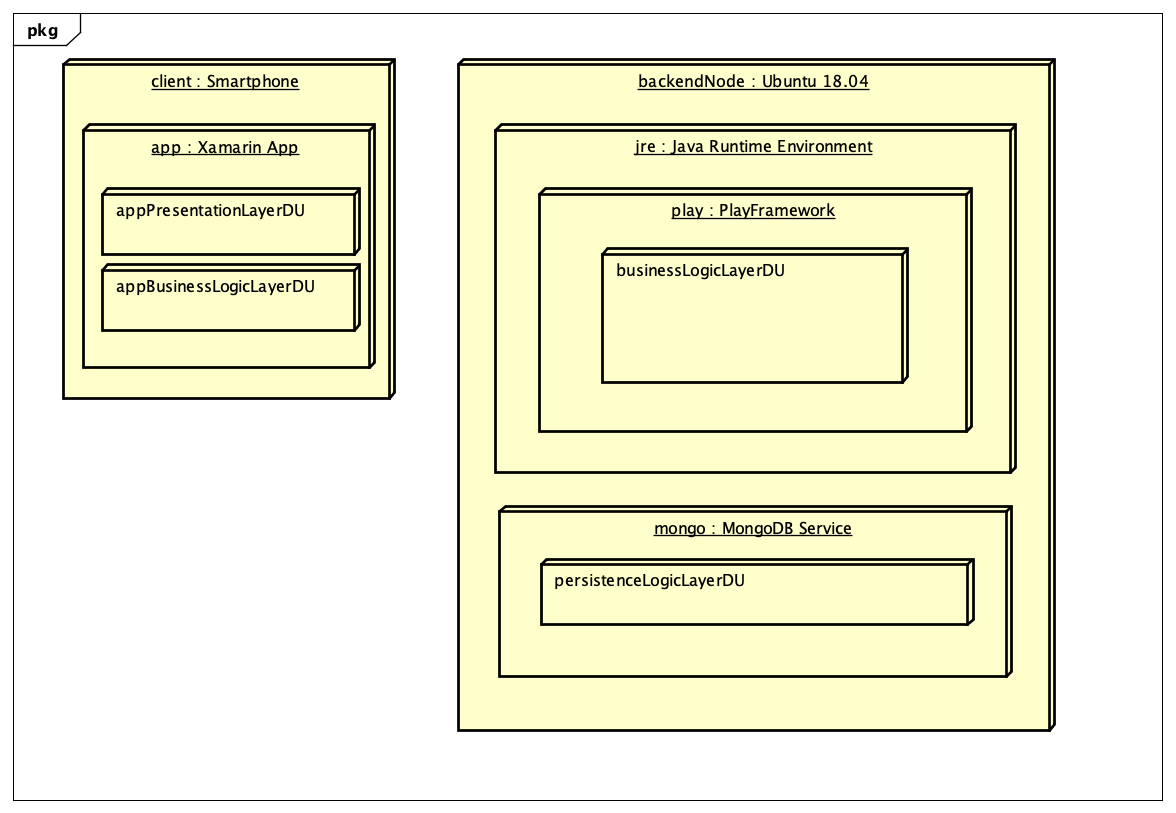
\includegraphics[width=1\linewidth]{img/deployment/DD_Methode635}
	\caption{Deploymentdiagramm BrainingOutOfBox}
	\label{fig:deployment-methode635}
\end{figure}

Beim Client handelt es sich um das Smartphone des jeweiligen Benutzers. Auf seinem Smartphone läuft die Xamarin App, welche wiederum die appPresentationLayerDU und die appBusinessLogicLayerDU hält.

Der BackendNode ist ein Ubuntu 18.04 auf dem ein Java Runtime Environment (JRE) installiert ist. Innerhalb der JRE läuft das PlayFramework, in dem wiederum die businessLogicLayerDU läuft.

Zudem ist auf dem BackendNode ein MongoDB Service installiert, welche  die persistenceLogicLayerDU beinhaltet.

\paragraph*{Komponenten}
Nachfolgend sind nochmals alle DeploymentUnits aufgelistet und kurz beschrieben.
\begin{description}[leftmargin=!,labelwidth=\widthof{\bfseries appBusinessLogicLayerDU}]
	\item[businessLogicLayerDU] Die businessLogicLayerDU enthält alle Komponenten, welche in Abbildung \ref{fig:architektur-methode635} in der Businesslogic-Schicht im PlayFramework eingezeichnet sind.
	\item[persistenceLogicLayerDU] Die persistenceLogicLayerDU beinhaltet alle Komponenten der Persistence-Schicht, welche in Abbildung \ref{fig:architektur-methode635} zu sehen ist.
	\item[appPresentationLayerDU] Die appPresentationLayerDU enthält alle Komponenten, welche in Abbildung \ref{fig:architektur-methode635} in der Präsentationsschicht liegen.
	\item[appBusinessLogicLayerDU] Die appBusinessLogicLayerDU enthält alle Komponenten, welche in Abbildung \ref{fig:architektur-methode635} in der Businesslogic-Schicht in der Xamarin App gezeichnet sind.
\end{description}
